\documentclass[chapters]{IEEEtran}
% \IEEEoverridecommandlockouts
% The preceding line is only needed to identify funding in the first footnote. If that is unneeded, please comment it out.
\usepackage{cite}
\usepackage{amsmath,amssymb,amsfonts}
\usepackage{algorithmic}
\usepackage{graphicx}
\usepackage{textcomp}
\usepackage{xcolor}
\usepackage{caption}

\def\BibTeX{{\rm B\kern-.05em{\sc i\kern-.025em b}\kern-.08em
    T\kern-.1667em\lower.7ex\hbox{E}\kern-.125emX}}

\usepackage{biblatex}

\graphicspath{ {./figures/} }
\addbibresource{reference.bib}

\begin{document}

\section{Literature Review}

\subsection{Transformers}
The 

\begin{figure}[!htb]
    \centering
        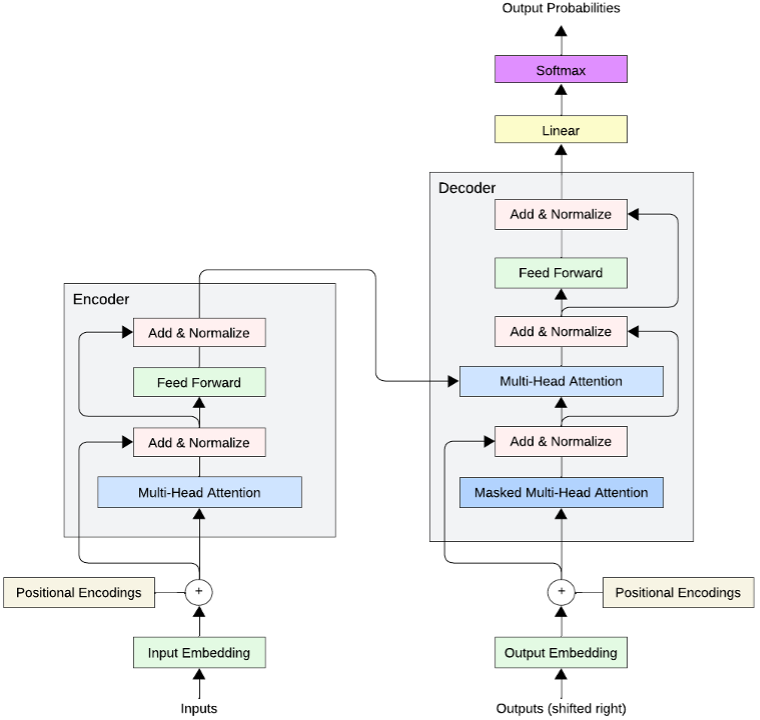
\includegraphics[width=0.75\linewidth]{figures/transformers_architecture.png}
        \caption{The transformer architecture}
\end{figure}

\subsection{Large Language Models (LLM)}

The are three different architectures for Large Language Models, encoder-only, decoder-only, and encoder-decoder. Each one has advantages on specific tasks.

\subsubsection{Encoder-only models}
These models are like BERT.
This type of model predict by masking specific words in a sentence.
The are better for classification and sentiment analysis.

\subsubsection{Decoder-only models}
For these model we have the well known GPT-3, Mistral, and LLaMa.
They receive one input and try to predict the entire text.
They are good for summarizing and text-generation.


\subsubsection{Encoder-Decoder models}
The encoder-decoder models are T5.
They mask entire sequences of text.
Good for translation and question and answering. \cite{9906925}

\subsection{Health Misinformation}

\printbibliography %Prints bibliography

\end{document}